% Article 1 manuscript — Springer Nature sn-article template (sn-mathphys-num style).
% Target journal: Minds and Machines (Springer).
\documentclass[pdflatex,sn-mathphys-num]{sn-jnl}

\usepackage{graphicx}
\usepackage{multirow}
\usepackage{amsmath,amssymb,amsfonts}
\usepackage{amsthm}
\usepackage{booktabs}
\usepackage{tabularx}
\usepackage{threeparttable}
\usepackage{xcolor}

\graphicspath{{figures/}}

\raggedbottom

\newtheorem{theorem}{Theorem}
\newtheorem{corollary}[theorem]{Corollary}

\begin{document}

\title[Ontological Innovation Limits in LLMs]{Operational Limits of Ontological Innovation in LLMs: Evidence from Controlled Sensory-Modality Generation}

\author*[1]{\fnm{Jarno} \sur{Matarmaa}}\email{iarnoolavi.matarmaa@urfu.ru}
% \author[1]{\fnm{Second} \sur{Author}}\email{author2@urfu.ru}

\affil*[1]{\orgdiv{Institute of Radio Electronics and Information Technologies}, \orgname{Ural Federal University}, \orgaddress{\city{Yekaterinburg}, \country{Russia}}}

\abstract{%
Contemporary large language models generate text that can appear conceptually novel, raising
the question of whether outputs reflect genuine ontological innovation---the introduction
of concepts that cannot be expressed as recombinations or transformations of training-derived
primitives---or sophisticated recombination within a fixed representational manifold. We test
this via a controlled experiment in an eight-modality sensory ontology. Seven language models
(\textit{N}\,=\,168 proposals; 24 runs each) were prompted to propose a genuinely new ninth
modality. Outputs were evaluated with four convergent methods: literature traceability
($\tau = 0.40$), structural decomposition, embedding-space convex-hull analysis, and continuous
novelty scoring. Results show a strict novelty rate of $\hat{p}_{\mathrm{novel}}=0.000$
(95\% CI: [0.000, 0.000]), traceability $\hat{p}_{\mathrm{traceable}}=0.982$, and 100\%
convex-hull membership under Sentence-BERT embeddings (3 PCA components). Structural
decomposition revealed three dominant failure modes: range extension (20.2\%), hybrid
combination (44.6\%), and functional recombination (17.9\%). Cross-model effects were moderate
($\eta^{2}=0.305$), but all models stayed within the same low-novelty regime, supporting a
constrained-manifold interpretation. Under the \emph{No New Basis Theorem}, gradient-descent
learning over fixed vocabularies cannot expand representational dimensionality beyond training
data. Current architectures therefore appear bounded by training-derived conceptual closures.
}

\keywords{ontological innovation, computational creativity, large language models,
          conceptual spaces, traceability analysis, representational constraints}

\maketitle

% =========================================================================
\section{Introduction}
\label{sec:intro}
% =========================================================================

The capacity to generate fundamentally new concepts---not merely recombinations of existing
ones---has long been considered a hallmark of human intelligence and a defining test of genuine
creativity.  As large language models (LLMs) achieve impressive performance on a broadening
range of generative tasks, a pressing question has emerged: do these systems exhibit
\emph{ontological innovation}, generating ideas that lie outside the conceptual closure of their
training environment, or do they operate as extremely capable recombinators constrained to a
fixed representational manifold?

This question has both philosophical and practical stakes.  Philosophically, it bears on the
computational theory of mind, the nature of creativity, and whether algorithmic systems can in
principle exceed the representational resources with which they were trained.  Practically, it
determines what roles LLMs can occupy in scientific discovery, design, and other domains where
genuinely new concepts---not just novel arrangements of existing ones---are required
\cite{kuhn1962structure}.

The challenge is that outputs from modern LLMs frequently \emph{appear} novel.  Proposals that
introduce unfamiliar terminology, combine concepts across disciplinary boundaries, or describe
mechanisms not explicitly present in any single training document can pass casual inspection as
genuinely creative \cite{wiggins2006preliminary,colton2012computational}.  Evaluating whether
such outputs constitute true conceptual innovation requires a controlled experimental setup and
rigorous multi-method analysis rather than surface-level assessment.

In this paper we report a focused empirical study designed to provide exactly this kind of
evaluation.  We use a multimodal sensory ontology---a well-defined, eight-modality conceptual
space representing biological and extended machine sensing---as the experimental universe.
This setup provides precise control: we know exactly which concepts exist in the training
context, enabling systematic investigation of whether AI-generated proposals lie outside the
defined space.  Seven contemporary LLMs were prompted to propose a \emph{ninth} sensory
modality, genuinely beyond any of the eight.  We evaluate their proposals through four
convergent methods that progressively sharpen the diagnostic picture.

Our main contributions are:

\begin{enumerate}
\item A controlled experimental paradigm for operationalising ontological innovation, grounded
      in a well-defined multi-modal sensory ontology that functions as an explicit training
      universe.
\item Multi-method evaluation combining literature traceability with calibrated thresholds,
      structural decomposition, embedding-space convex-hull analysis, and continuous novelty
      scoring, providing convergent evidence without reliance on subjective expert judgment.
\item Systematic empirical evidence that seven state-of-the-art LLMs produce zero strictly
      novel proposals across 168 evaluated outputs, with near-saturated traceability to known
      conceptual material.
\item Formal grounding through the \emph{No New Basis Theorem}, relating observed empirical
      constraints to architectural properties of gradient-descent-trained neural networks.
\end{enumerate}

The paper is organised as follows.  Section~\ref{sec:related} reviews related work on
computational creativity and representational limits.  Section~\ref{sec:methods} describes the
dataset, task, models, and evaluation procedures.  Section~\ref{sec:results} presents the
results across all evaluation methods.  Section~\ref{sec:discussion} interprets the findings
and Section~\ref{sec:limits} discusses limitations.

% =========================================================================
\section{Background and Related Work}
\label{sec:related}
% =========================================================================

\subsection{Boden's Creativity Taxonomy}

The dominant framework for analysing machine creativity is Margaret Boden's tripartite
taxonomy \cite{boden2004creative}, which distinguishes outputs based on their relationship to
the conceptual space from which they arise.  \emph{Combinational creativity} produces novel
combinations of familiar ideas---poetic metaphors, analogies, conceptual blends.
\emph{Exploratory creativity} systematically searches well-defined conceptual spaces to find
previously unvisited regions.  \emph{Transformational creativity}, the most radical category,
modifies the conceptual space itself by relaxing or changing its defining constraints.

Research on AI systems has demonstrated substantial competence at combinational and
exploratory creativity \cite{hofstadter1995fluid,cope1996experiments}.  Systems such as
Copycat, JAPE, and AARON can generate outputs that human evaluators judge as genuinely
surprising and apt within their respective domains.  Robust transformational creativity,
however, remains rare: most documented examples involve superficial parameter modifications
rather than fundamental reconceptualisation \cite{boden2004creative}.

Wiggins \cite{wiggins2006preliminary} introduced a formal framework for evaluating creativity
claims and identified a ``framing'' problem: systems appear to transform their conceptual space
while actually operating within an implicitly broader space defined by human designers.  This
critique applies with particular force to contemporary LLMs, whose training corpora implicitly
define a vast but still finite conceptual universe.

\subsection{Our Extension: Ontological Creativity}

We argue that a fourth category, which we term \emph{ontological creativity}, is needed to
capture the most radical form of conceptual innovation.  Transformational creativity modifies
operators $\Omega$ or relations $\mathcal{E}$ within a conceptual space $\mathcal{C} = (V,
\mathcal{E}, \Phi, \Omega)$; ontological creativity introduces new \emph{primitive} concepts
$v' \in V'$ where $V' \not\subset V$ and critically $V'$ cannot be expressed as
$\Omega(V)$ for any existing operators.

This distinction maps onto Ryle's philosophical notion of category mistakes
\cite{ryle1949concept}: ontological creativity involves recognising that existing categories
are insufficient and proposing new ones that cannot be defined by recombining or transforming
current primitives.  Einstein's reconceptualisation of absolute simultaneity as a category
error, leading to a revised ontology of relativistic spacetime, exemplifies this form of
creativity.  Generating a genuinely new sensory modality would be analogous: not an extension
or hybridisation of existing ones, but a proposal for a sensing type with a physical basis and
information content that cannot be expressed as a composition of the existing eight.

\subsection{Formal Representational Constraints}

The computational theory of mind \cite{turing1936computable,godel1931formal} and its critics
\cite{searle1980minds,penrose1990emperors,dreyfus1972computers} have long debated whether
algorithmic systems face principled limits on what they can represent and understand.  Recent
work in mechanistic interpretability provides empirical traction on this question by revealing
that generation in transformer-based LLMs proceeds through retrieval and interpolation among
training examples rather than through any inference mechanism that could introduce entirely new
primitives \cite{brown2020language,elhage2021mathematical}.  The transformer architecture
\cite{vaswani2017attention} encodes all knowledge implicitly in weights learned from
distributional co-occurrence, which grounds the output space in the training vocabulary of
concepts.  G{\"a}rdenfors's conceptual-spaces formalism \cite{gardenfors2000conceptual}
provides complementary geometric intuition: a learned concept lives as a region in a quality
space, and generating a new concept outside all existing regions requires an external
basis vector not present in the training data.

We formalise the core constraint as the \emph{No New Basis Theorem}: for any neural
architecture $\mathcal{A}$ operating over representation space $\mathbb{R}^{d}$ with
generative process $G\colon \mathbb{R}^{d} \to \mathbb{R}^{d}$ learned from training data
$\mathcal{D} = \{x_1,\ldots,x_N\}$, all generated outputs $x' = G(z)$ lie within $\mathcal{M}'$,
a continuous deformation of $\mathcal{M} = \mathrm{span}(\{x_1,\ldots,x_N\})$ satisfying
$\dim(\mathcal{M}') \leq \dim(\mathcal{M})$.  Ontological novelty would require expanding the
basis of $\mathcal{M}$, which no internal generative mechanism can achieve without
architectural or data augmentation.

This theorem explains why even highly capable models that produce surprising combinations
remain formally constrained to the conceptual universe their training data defines.  Our
empirical study provides a controlled test of whether this theoretical constraint manifests
behaviorally.

\subsection{Evaluation Challenges in Computational Creativity}

A persistent methodological challenge in computational creativity research is evaluation
\cite{wiggins2006preliminary,colton2012computational}.  Human expert judgments are subjective,
difficult to reproduce, and sensitive to framing.  Recent studies show that LLMs can
achieve human-level performance on divergent-thinking tasks such as the Alternative Uses Test
\cite{stevenson2022gpt}, but scoring quality depends strongly on the evaluation metric
\cite{organisciak2023beyond}.  Recent 2024--2026 work further confirms metric sensitivity and
proposes newer creativity-evaluation protocols for LLMs, including human-comparative,
temperature-sensitivity, and model-guided creativity-judging paradigms
\cite{zhao2024assessing,wang2024canai,peeperkorn2024temperature,bellemare2024divergent,ismayilzada2024shortstory,nakajima2026beyonddivergent,olson2024steering}.  Our multi-method approach---traceability
search, structural decomposition, embedding-space geometry, and continuous scoring---provides
convergent automated evidence that can be replicated and extended.  Calibrated traceability
thresholds replace arbitrary cut-offs with empirically justified operating points.

% =========================================================================
\section{Materials and Methods}
\label{sec:methods}
% =========================================================================

\subsection{The Multimodal Sensory Ontology}

The experimental universe consists of eight sensory modalities, each defined by a physical
basis, an information channel, and a functional role in an agent's interaction with its
environment (Table~\ref{tab:modalities}).  Modalities span biological human senses and
extended machine-sensing capabilities:

\begin{table}[tp]
\caption{Eight-modality sensory ontology used as the experimental universe.
Each modality is defined by its physical basis, representational dimensionality, and
functional role.}
\label{tab:modalities}
\begin{tabularx}{\textwidth}{lXXr}
\toprule
\textbf{Modality} & \textbf{Physical basis} & \textbf{Functional role} & \textbf{Dim.} \\
\midrule
Visual       & EM spectrum 300--1000\,nm (5\,nm steps) & Scene and object recognition & 140 \\
Auditory     & Pressure waves 1\,Hz--100\,kHz (128-bin FFT) & Sound source localisation & 128 \\
Tactile      & Mechanical vibrations 5--800\,Hz & Surface texture and pressure & 32 \\
Olfactory    & Chemical categories (10 classes) & Substance identification & 10 \\
Gustatory    & Taste dimensions (sweet/sour/salty/bitter/umami) & Ingestion guidance & 5 \\
Proprioceptive & 20 joint angles + 10 muscle tensions & Body-state estimation & 30 \\
Vestibular   & 3-axis acceleration + 3-axis angular velocity & Balance and motion & 6 \\
Interoceptive & HR, respiration, skin conductance, temperature, hunger, thirst, fatigue, pain & Homeostatic regulation & 8 \\
\midrule
\multicolumn{3}{l}{\textit{Total feature dimensionality per timestep}} & 359 \\
\bottomrule
\end{tabularx}
\end{table}

The full dataset contains 5,000 training, 1,000 validation, and 1,000 test examples, each
representing a 60-second episode at 1\,Hz sampling (21,540 data points per example) drawn from
seven everyday scenarios (walking, running, sitting, eating, drinking, listening, viewing).  An
explicit machine-readable ontology layer documents the physical basis, information content, and
functional role of each modality, enabling automated evaluation.

\subsection{Task Definition and Prompt Contract}

Each model was asked to \emph{propose a ninth sensory modality that is genuinely new and not
reducible to combinations, extensions, or transformations of the existing eight}.  Proposals
were required to specify: (1) the physical phenomenon to be sensed, (2) the information channel
and encoding, and (3) the functional difference from existing modalities.  The complete ontology
table (Table~\ref{tab:modalities}) was provided in structured tabular format alongside a
natural-language description of each modality.

Prompts were designed to be task-neutral---they did not suggest what kinds of answers would or
would not qualify as novel, to avoid anchoring models toward specific response types.  Twenty-four
independent runs were collected from each of seven models, yielding $N = 7 \times 24 = 168$
proposals in total.

\subsection{Models and Implementation}

Seven state-of-the-art models were evaluated: GPT-5.2 \cite{openai2023gpt4}, Claude-3.7-Sonnet,
Gemini-3.1-Pro-Preview \cite{gemini15_2024}, LLaMA-3.3-70B-Instruct \cite{llama3herd_2024},
DeepSeek-v3.2 \cite{deepseekv3_2024,deepseekr1_2025}, Mistral-Large \cite{mixtral2024}, and Perplexity
Sonar Pro, accessed via the OpenRouter, Perplexity, and Mistral APIs.  All runs used
temperature $T=0.7$; the Perplexity API does not support temperature adjustment and was
operated at provider defaults.  System prompts were crafted to neutrally present the task
without introducing bias toward particular answer types.

\subsection{Evaluation Protocol}

\paragraph{Literature traceability.}
Each proposal was matched against a curated scholarly corpus of 125 documents covering sensory
biology, robotics sensing, and computational neuroscience, using cosine similarity over
Sentence-BERT embeddings \cite{reimers2019sentencebert}.  A proposal is classified as
\emph{traceable} if its best-match similarity exceeds threshold $\tau$.

Threshold selection followed an explicit calibration step.  Three candidate operating points
($\tau \in \{0.30, 0.40, 0.50\}$) were compared on the full response--corpus similarity
distribution.  At $\tau=0.30$, every proposal was traceable (mean 23.7 matching documents per
proposal), providing no discrimination.  At $\tau=0.50$, only 64.9\% of proposals were
traceable (mean 1.24 matching documents), indicating over-pruning.  The intermediate value
$\tau=0.40$ was retained as the best-justified operating point: 98.2\% traceability with a
mean of 7.36 above-threshold matches per proposal, preserving discriminability while avoiding
either degenerate extreme.

\paragraph{Structural decomposition.}
Each proposal was analysed for whether its key claims can be expressed using only the eight
training primitives through: (i) range extension (preserving the sensing type while shifting
its physical parameter range), (ii) hybrid combination (combining features from two or more
existing modalities), or (iii) functional recombination (repurposing an existing sensing
mechanism for a different functional role).  Proposals not fitting any category were labelled
\emph{structurally novel}.

\paragraph{Embedding-space convex-hull analysis.}
Sentence-BERT embeddings were computed for each proposal and for the eight training-modality
descriptions.  Principal component analysis reduced both sets to three components; convex-hull
membership was computed in 3D using half-space equations with numerical tolerance.  A proposal
classified as \emph{outside} the hull would occupy a semantically isolated region suggesting
basis expansion beyond the training ontology.

\paragraph{Continuous novelty scoring.}
A continuous novelty score $s \in [0,1]$ was computed for each proposal by combining
structural novelty sub-scores: (i) absence from structural decomposition categories, (ii)
inverse of maximum cosine similarity to training modalities, and (iii) geometric distance from
the convex-hull boundary.  Proposals with $s \geq 0.5$ were classified as strictly novel under
this operational threshold.

% =========================================================================
\section{Results}
\label{sec:results}
% =========================================================================

\subsection{Primary Outcomes}

The aggregate strict novelty rate was $\hat{p}_{\mathrm{novel}} = 0.000$ (95\% CI: [0.000,
0.000]; $N=168$).  No proposal satisfied the strict novelty criterion $s \geq 0.5$.  The mean
continuous novelty score was $\hat{\mu}_{\mathrm{continuous}} = 0.059$ (SD $= 0.031$),
indicating weak novelty signal without threshold-level novelty events across any model or run.

Under the calibrated traceability threshold $\tau = 0.40$, the traceability rate was
$\hat{p}_{\mathrm{traceable}} = 0.982$ (95\% CI: [0.962, 1.000]); 165 of 168 proposals had a
best-match cosine similarity above threshold, with a mean best-match score of 0.528 across all
proposals.  Of the 165 traceable proposals, all 165 were matched to sources from the
strong-evidence tier of the corpus.

Figure~\ref{fig:classification} presents the dominant classification split: traceable/non-novel
outputs are overwhelmingly prevalent across all models.

\begin{figure}[tp]
\centering
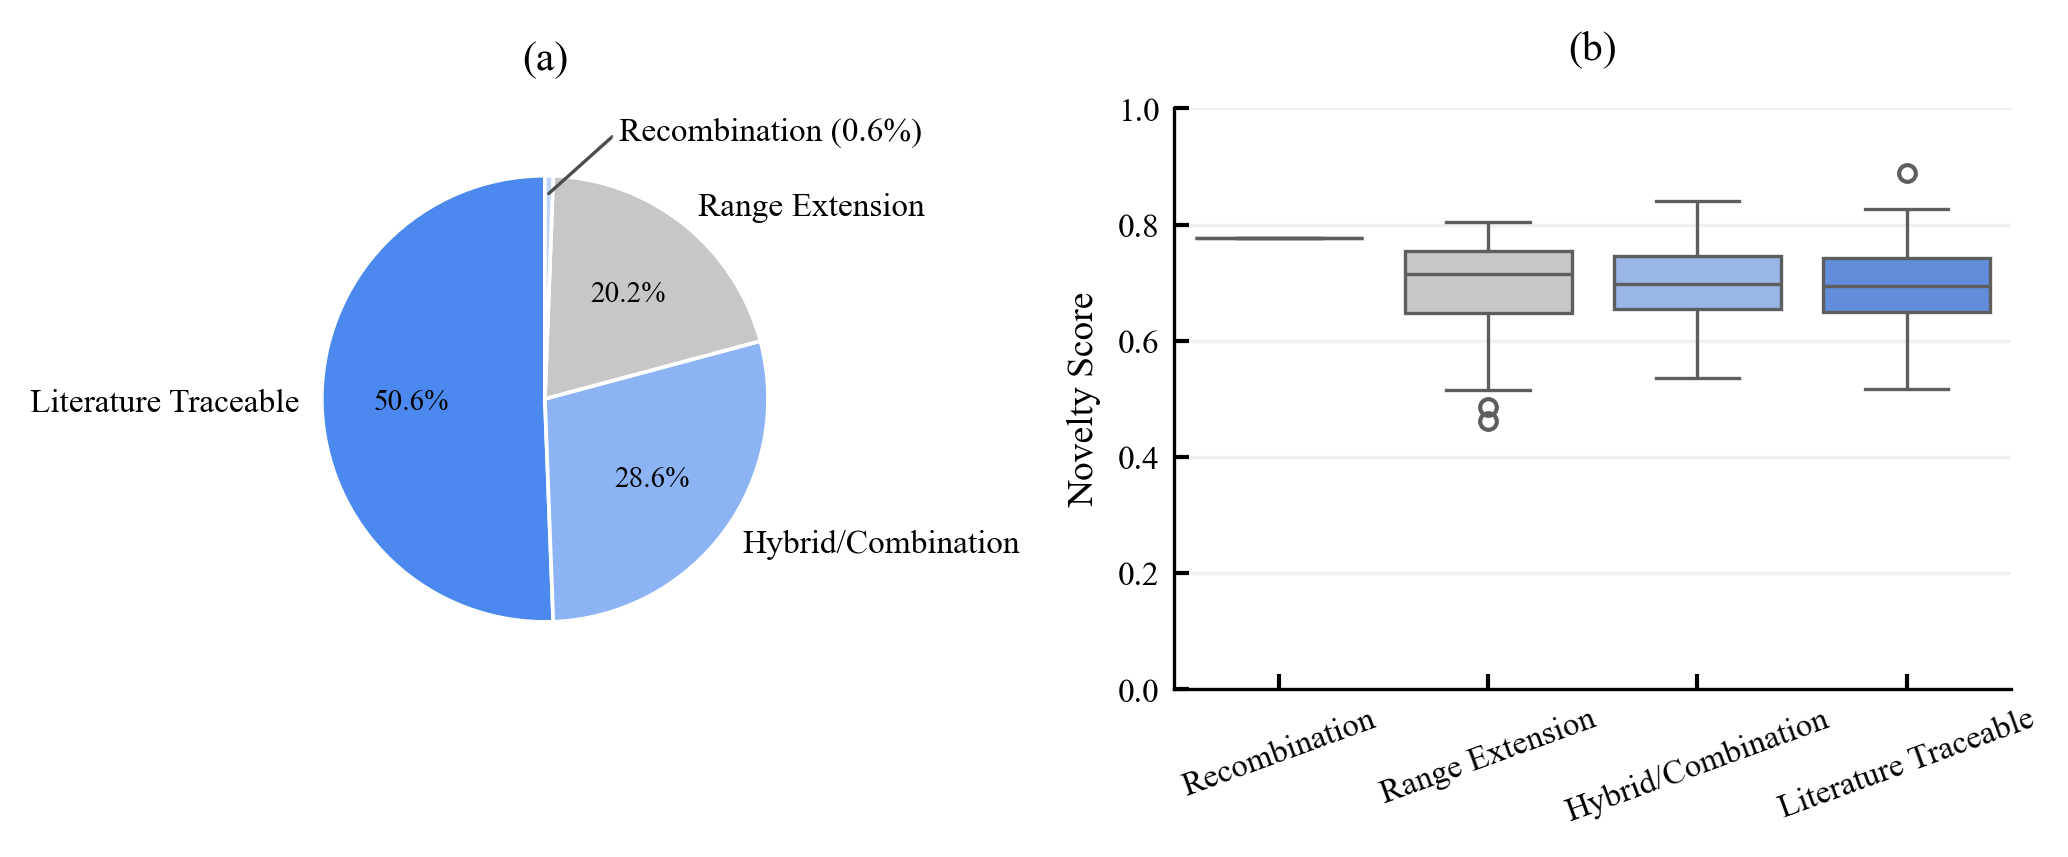
\includegraphics[width=\textwidth]{t1_classification_summary.png}
\caption{Classification summary ($N=168$ proposals, seven models).
(a)~Distribution of classification outcomes; the distribution is dominated by traceable
categories consistent with low operational ontological novelty under calibrated thresholds.
(b)~Novelty score distributions by classification category shown as box plots.}
\label{fig:classification}
\end{figure}

\subsection{Structural Decomposition}

Of the 168 proposals, 88 (52.4\%) were structurally decomposable into training-ontology
primitives.  Three failure modes account for the decomposable proposals:

\begin{itemize}
\item \textbf{Range extension} (34 cases, 20.2\%): proposals that extend the physical
      parameter range of an existing modality (e.g., far-infrared thermal sensing as an
      extension of visual EM-band coverage, or infrasound-extended auditory detection).
\item \textbf{Hybrid combination} (75 cases, 44.6\%): proposals combining features from two or
      more existing modalities (e.g., combined tactile-proprioceptive ``haptic flow'' sensing,
      or olfactory-gustatory integration).
\item \textbf{Functional recombination} (30 cases, 17.9\%): proposals repurposing an existing
      sensing mechanism for a different functional role (e.g., using interoceptive signals for
      external-environment monitoring rather than homeostatic regulation).
\end{itemize}

The remaining 80 proposals (47.6\%) were not fully decomposable through the three named
categories but nonetheless fell within the traceability threshold, indicating semantic
proximity to known concepts even without a simple structural decomposition path.

Figure~\ref{fig:frontier_bands} shows novelty-frontier band assignments by model, confirming
that the low-novelty/high-traceability pattern holds architecture-wide rather than being driven
by a single underperforming model.  Figure~\ref{fig:frontier_decomp} further illustrates that
most proposals fail multiple frontier criteria simultaneously, supporting a coupled-constraint
interpretation.

\begin{figure}[tp]
\centering
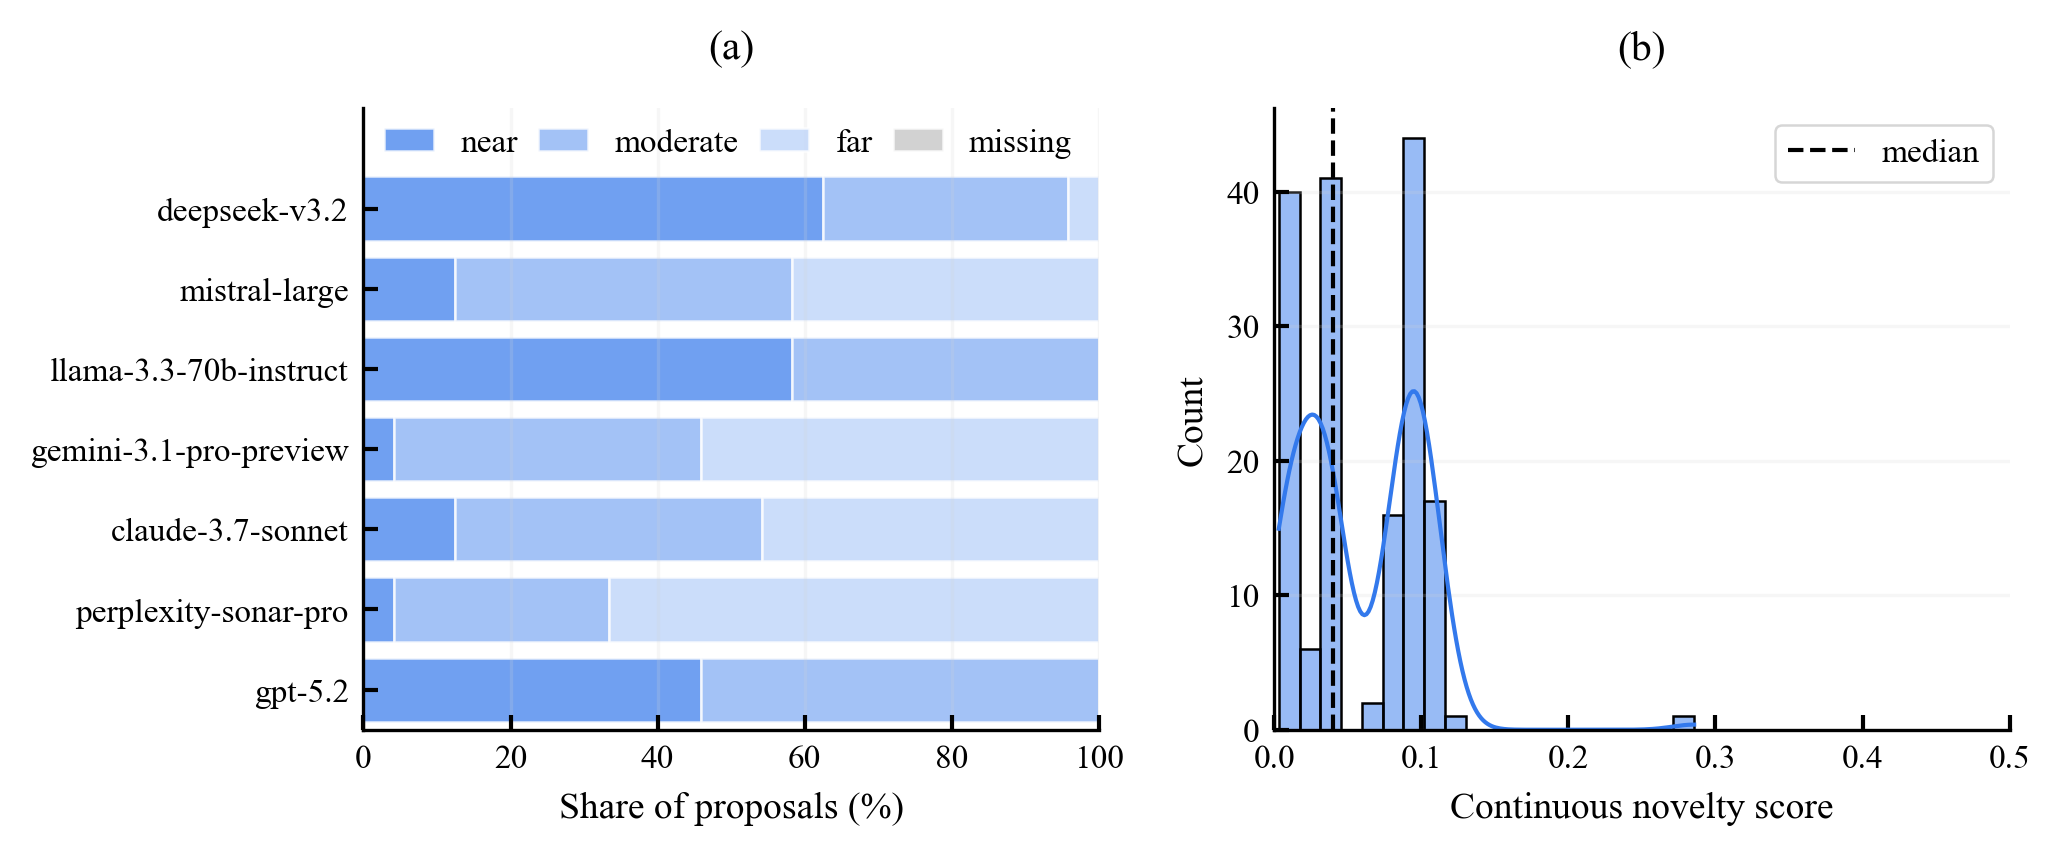
\includegraphics[width=\textwidth]{t1_novelty_frontier_bands_by_model.png}
\caption{Novelty-frontier band assignments and score distribution.
(a)~Band assignment by model: responses are concentrated in low-novelty and frontier-proximal
bands across all seven architectures, indicating architecture-independent constraint patterns
rather than isolated model failures.
(b)~Overall continuous novelty score distribution with KDE overlay; dashed line marks the median.}
\label{fig:frontier_bands}
\end{figure}

\begin{figure}[tp]
\centering
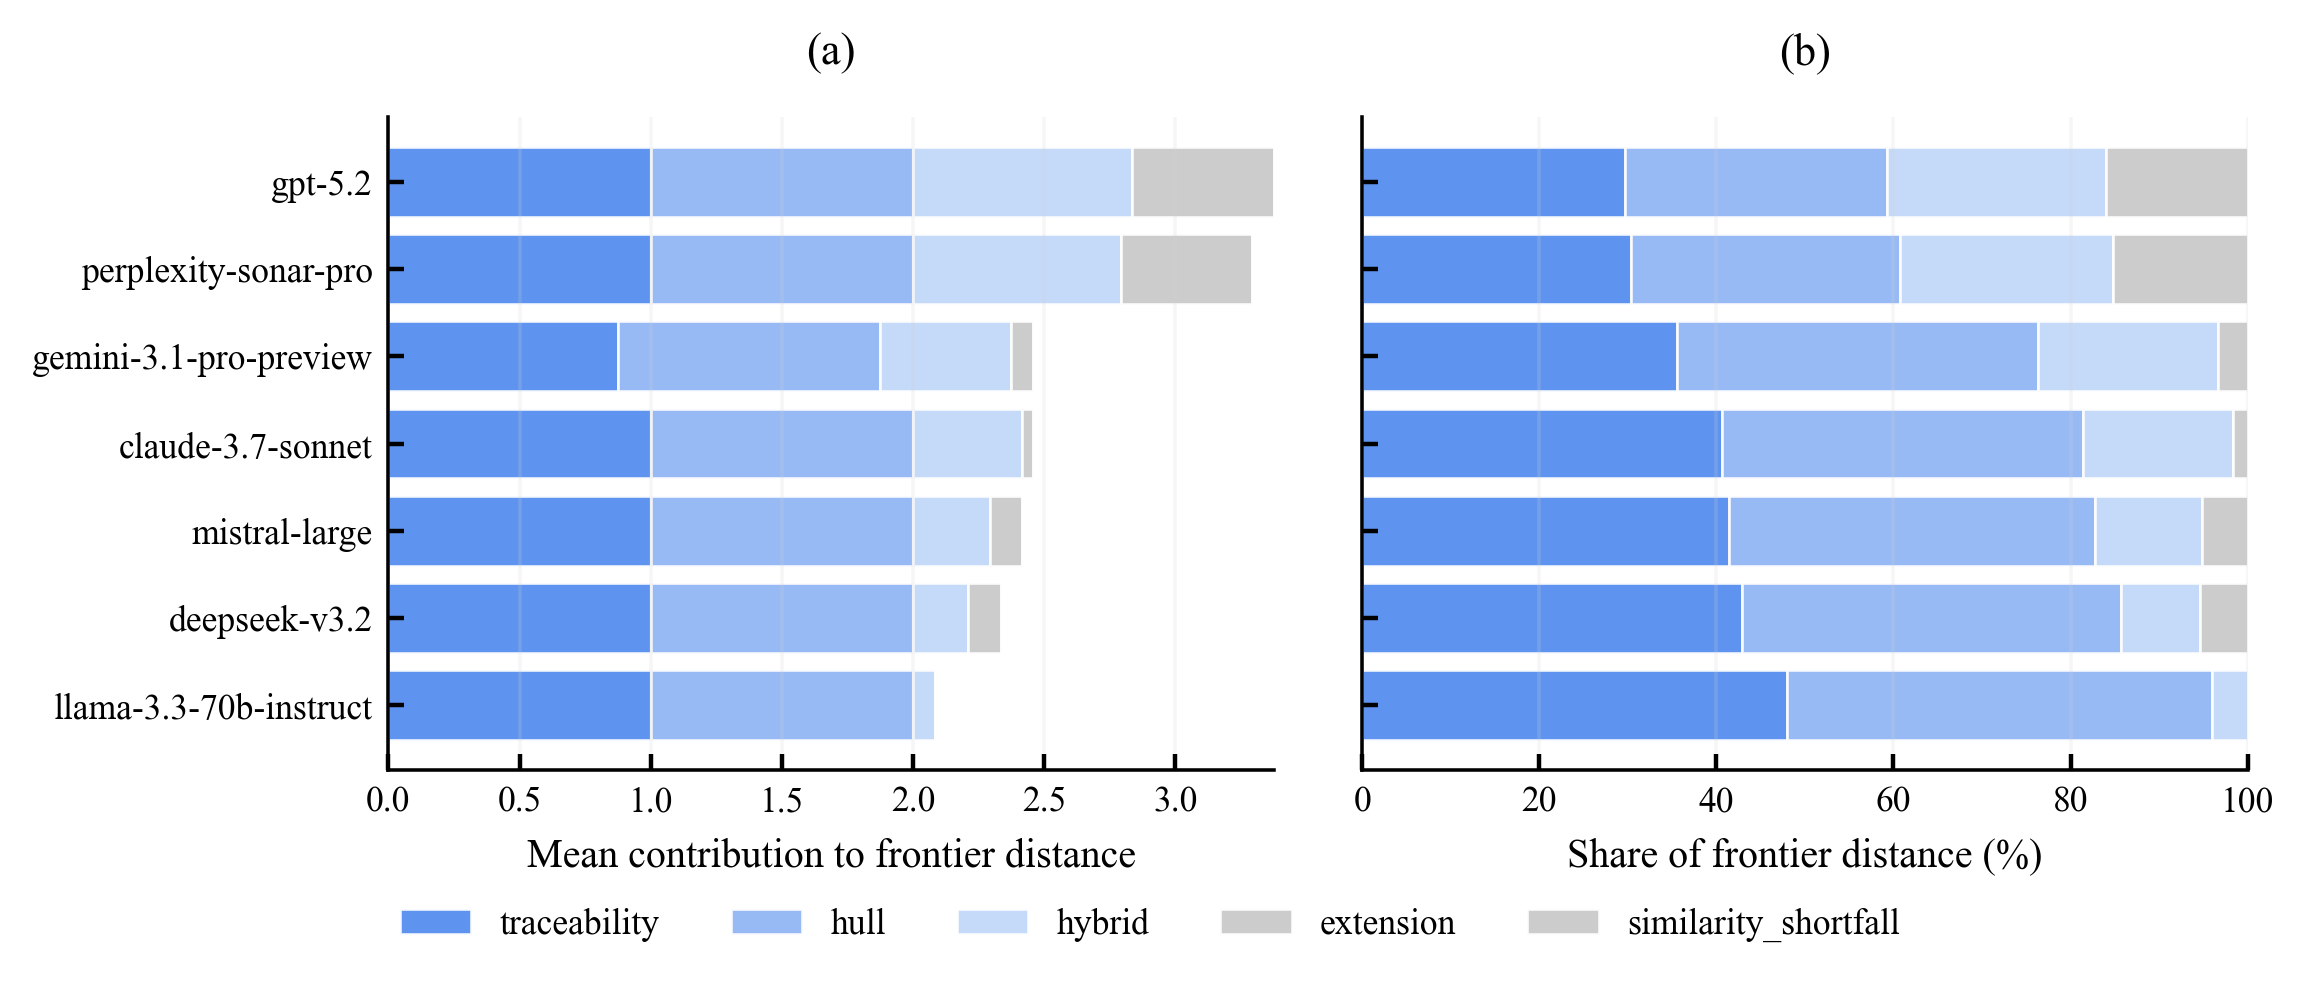
\includegraphics[width=\textwidth]{t1_novelty_frontier_decomposition_by_model_combined.png}
\caption{Novelty-frontier criterion decomposition by model.
(a)~Absolute mean contribution of each criterion to overall frontier distance.
(b)~Relative share (\%) of frontier distance per criterion.
Both panels confirm that most responses violate multiple criteria simultaneously, supporting
a coupled-constraint interpretation of low ontological novelty.}
\label{fig:frontier_decomp}
\end{figure}

\subsection{Embedding-Space Geometry}

All 168 proposals (100\%) were classified as inside the 3D convex hull of training-modality
embeddings.  Proposal markers cluster in the interior region of the training manifold; no
proposal occupies a semantically isolated region that would suggest basis expansion beyond the
training ontology.

The mean cosine similarity between each proposal and its closest training modality was
$\bar{d} = 0.305$ (SD $= 0.078$), indicating substantial semantic overlap with training
concepts.  Figure~\ref{fig:embedding} presents the embedding-space analysis with proposals
visualised in the first two principal components and the 3D hull boundary shown as a visual
aid.

\begin{figure}[tp]
\centering
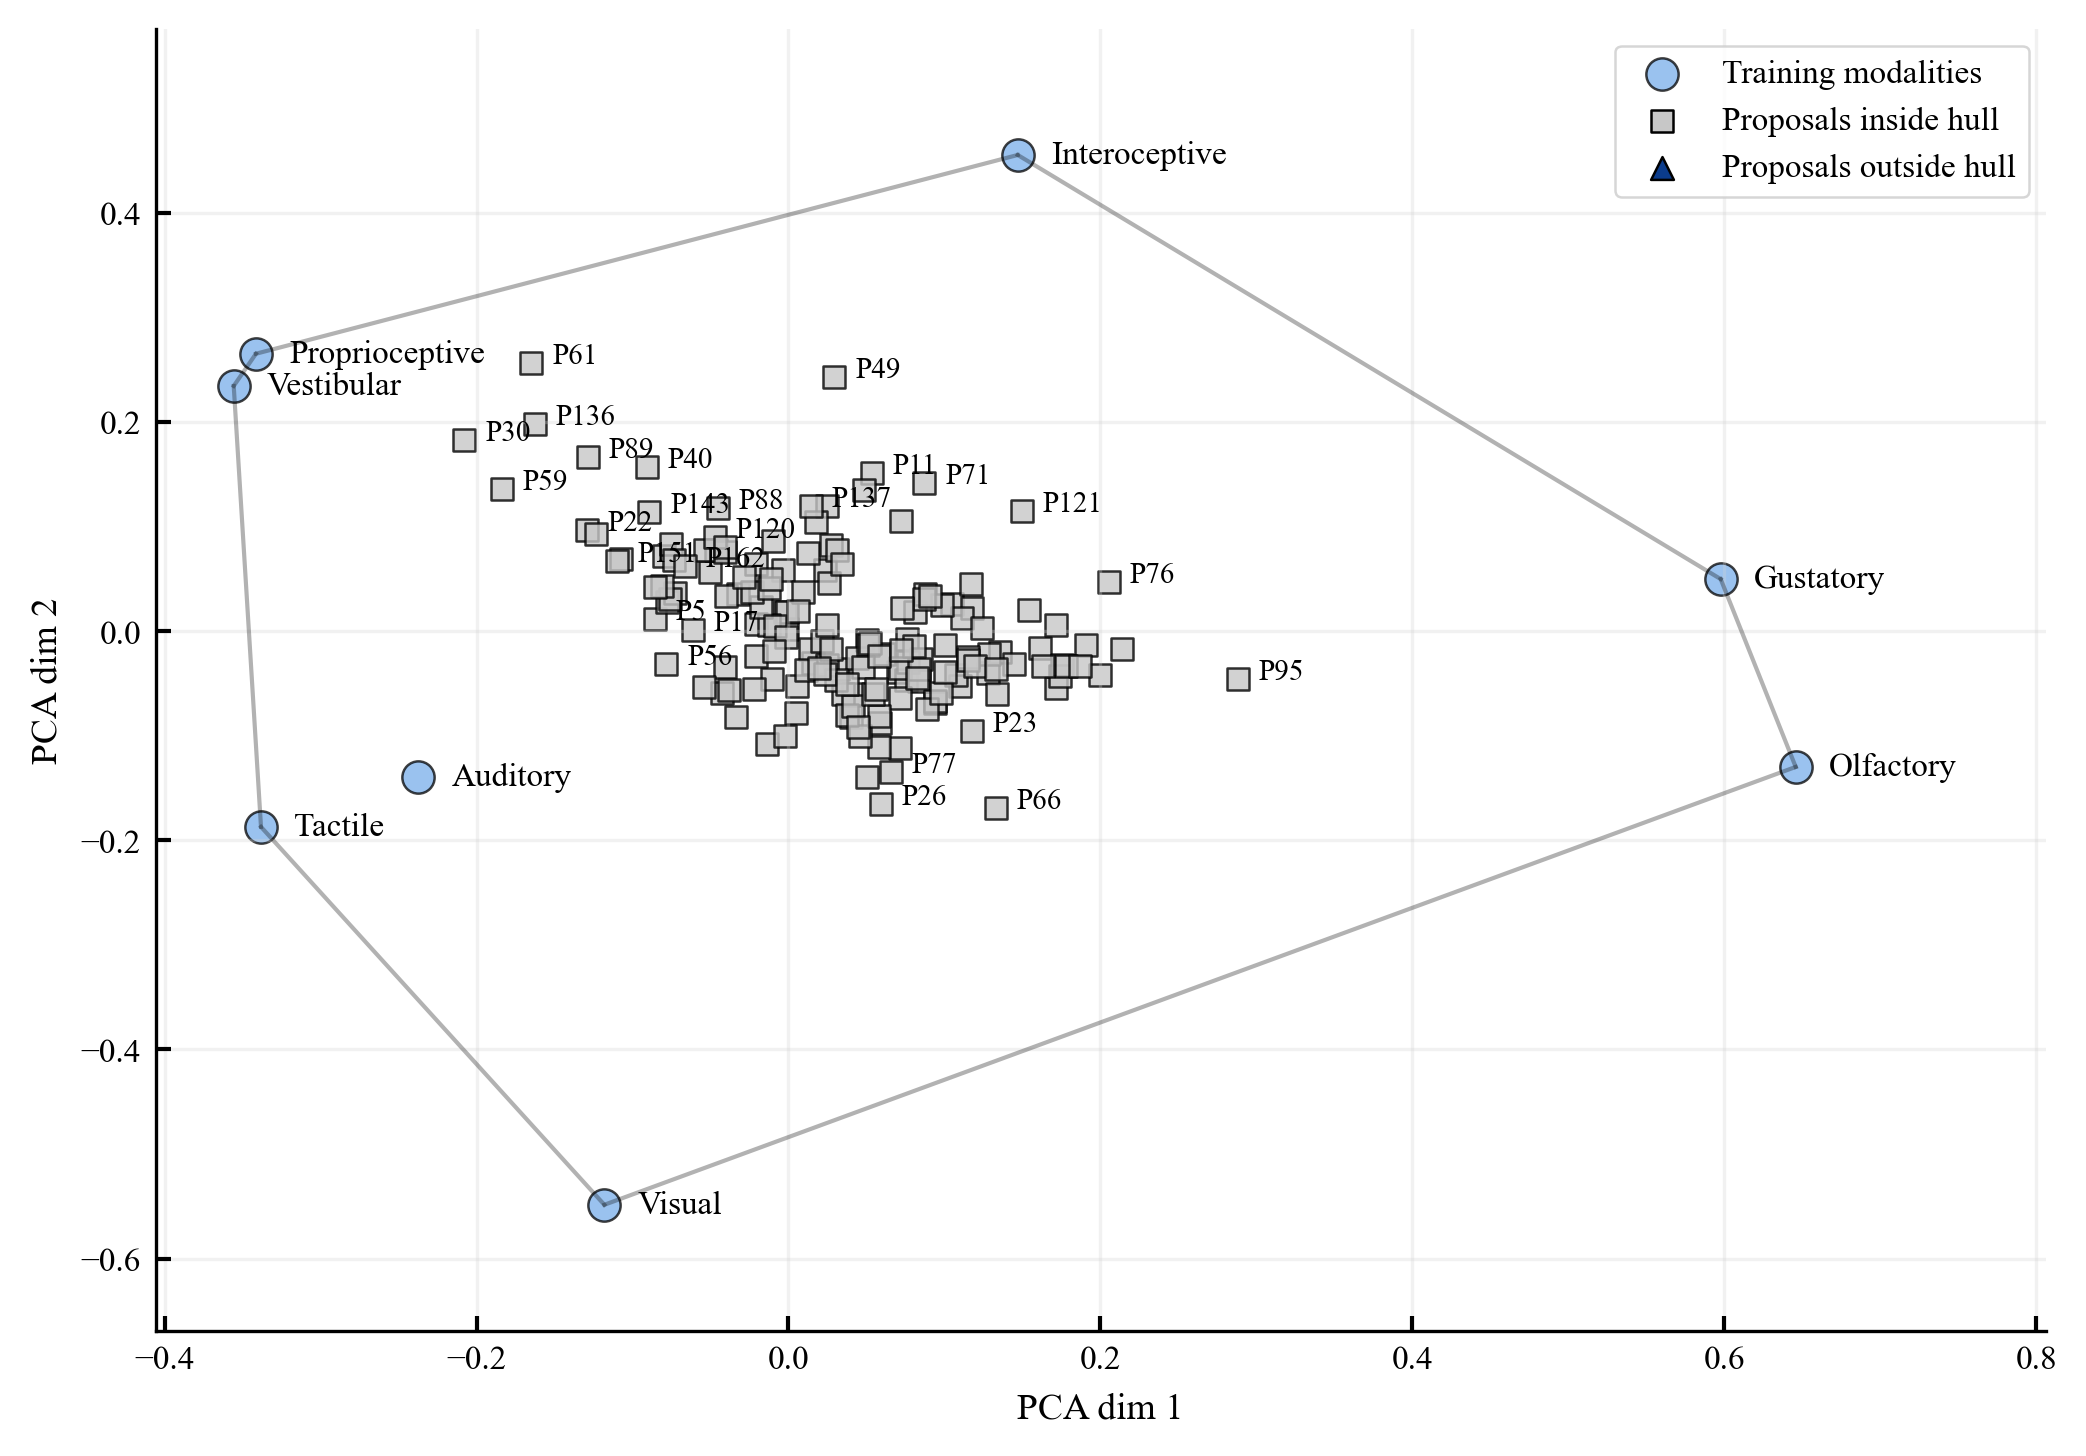
\includegraphics[width=\textwidth]{t1_embedding_space_analysis.png}
\caption{Embedding-space analysis for proposals and training modalities. Convex-hull
membership is computed in PCA-reduced 3D space; the 2D boundary shown is illustrative only.
All 168 proposal markers cluster near the interior of the training manifold---none escape to
a semantically isolated region.}
\label{fig:embedding}
\end{figure}

Figure~\ref{fig:similarity_heatmap} provides the aggregated cosine-similarity heatmap of
proposed modalities against the eight training modalities, reaching the same conclusion from a
complementary metric: every proposal records elevated similarity to one or more training
modalities, with no proposal showing uniformly low similarity across all eight.

\begin{figure}[tp]
\centering
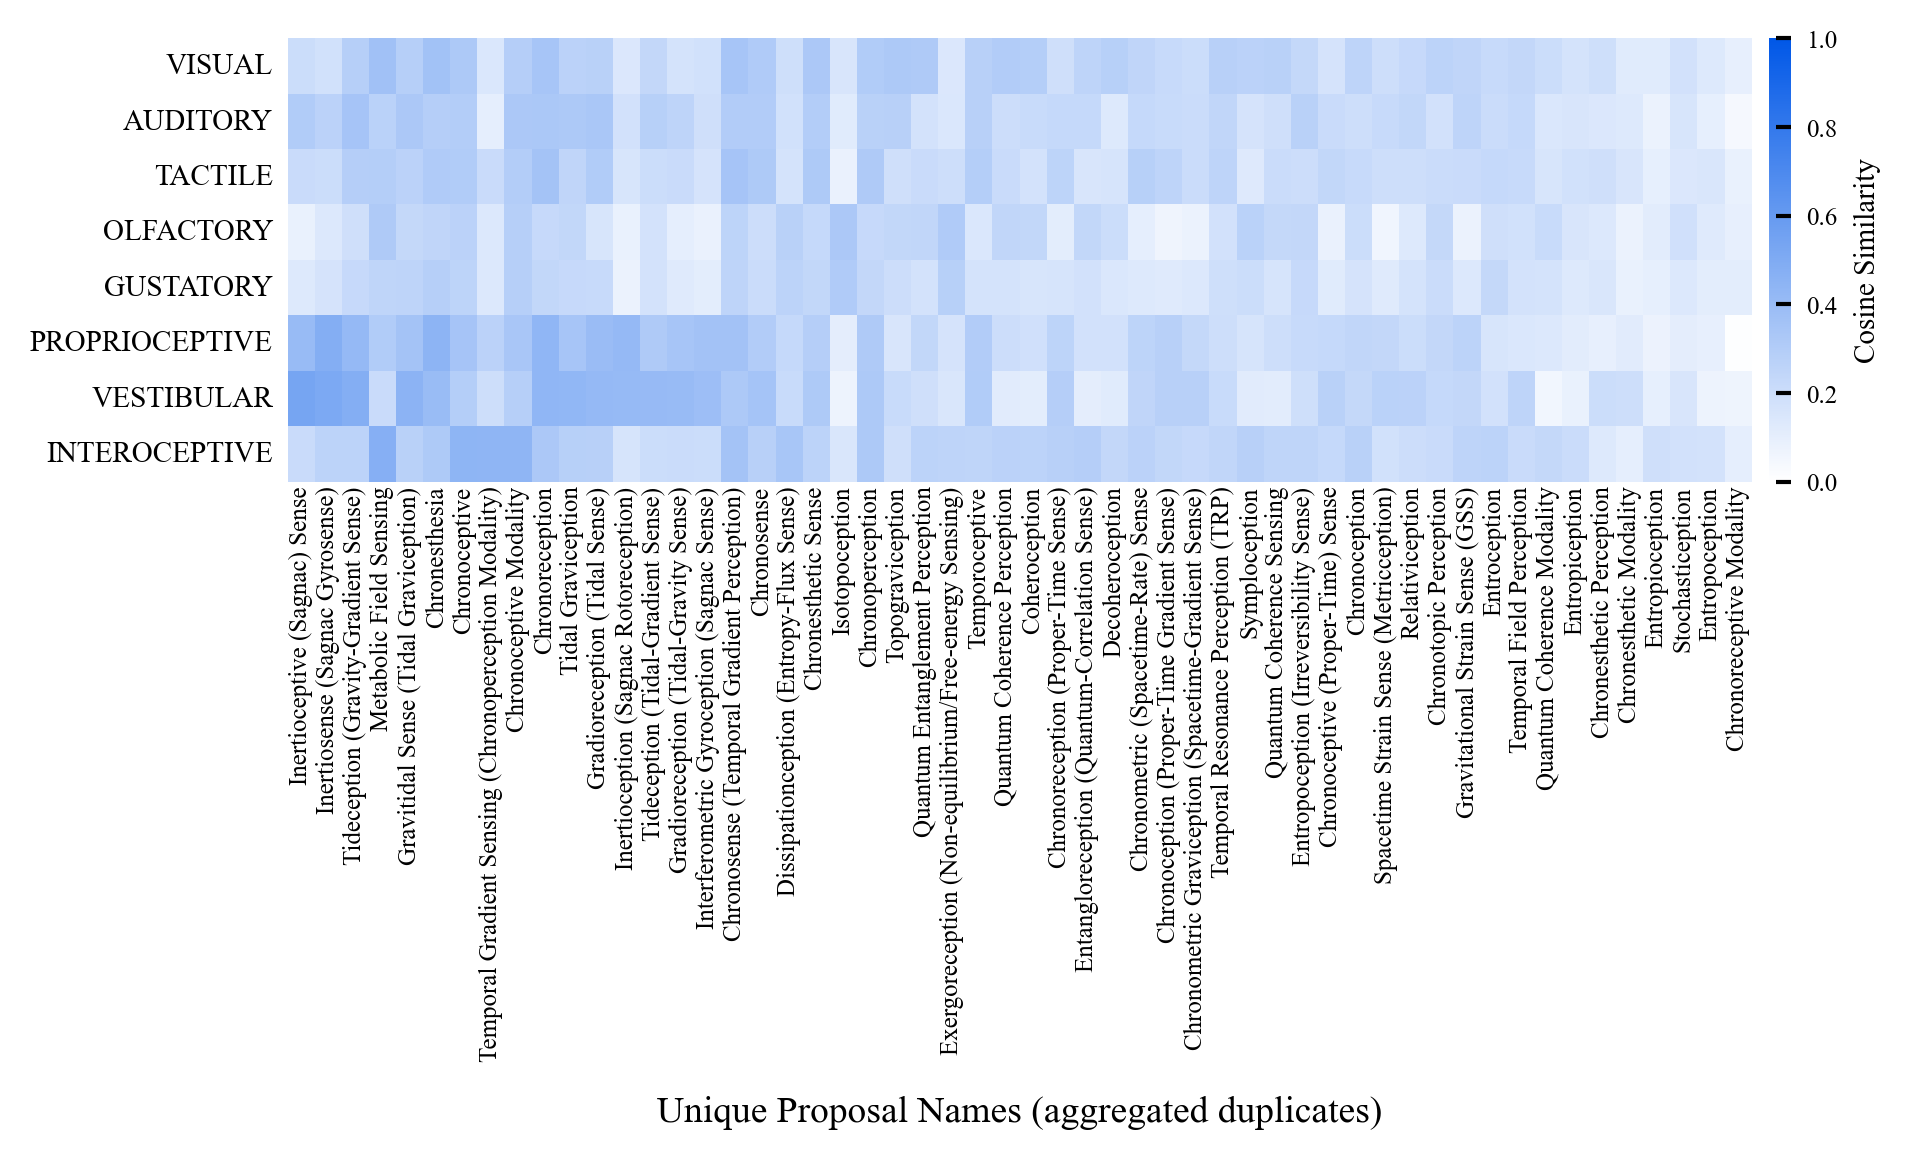
\includegraphics[width=\textwidth]{t1_similarity_heatmap_v1_optionA_aggregated.png}
\caption{Aggregated cosine similarity of proposed modalities to the eight training modalities.
Concentration of similarity values confirms the traceability finding: no proposal is
simultaneously dissimilar from all eight training types.}
\label{fig:similarity_heatmap}
\end{figure}

\subsection{Cross-Model Comparison}

The model effect on the primary novelty metric was moderate: one-way ANOVA yielded
$\eta^{2} = 0.305$, indicating non-trivial between-model variance in raw scores.  Nonetheless,
all seven models remained within the same low-novelty/high-traceability regime; no model
produced proposals classified as strictly novel, and no model achieved a mean continuous
novelty score exceeding $\mu = 0.12$.

Figure~\ref{fig:canonical_heatmap} shows that between-model variation takes the form of
different \emph{preferences among known canonical families} rather than emergence of
structurally new families: some models more frequently produced range-extension proposals while
others favoured hybrid combinations, but neither pattern represents departure from the
training-derived manifold.

\begin{figure*}[tp]
\centering
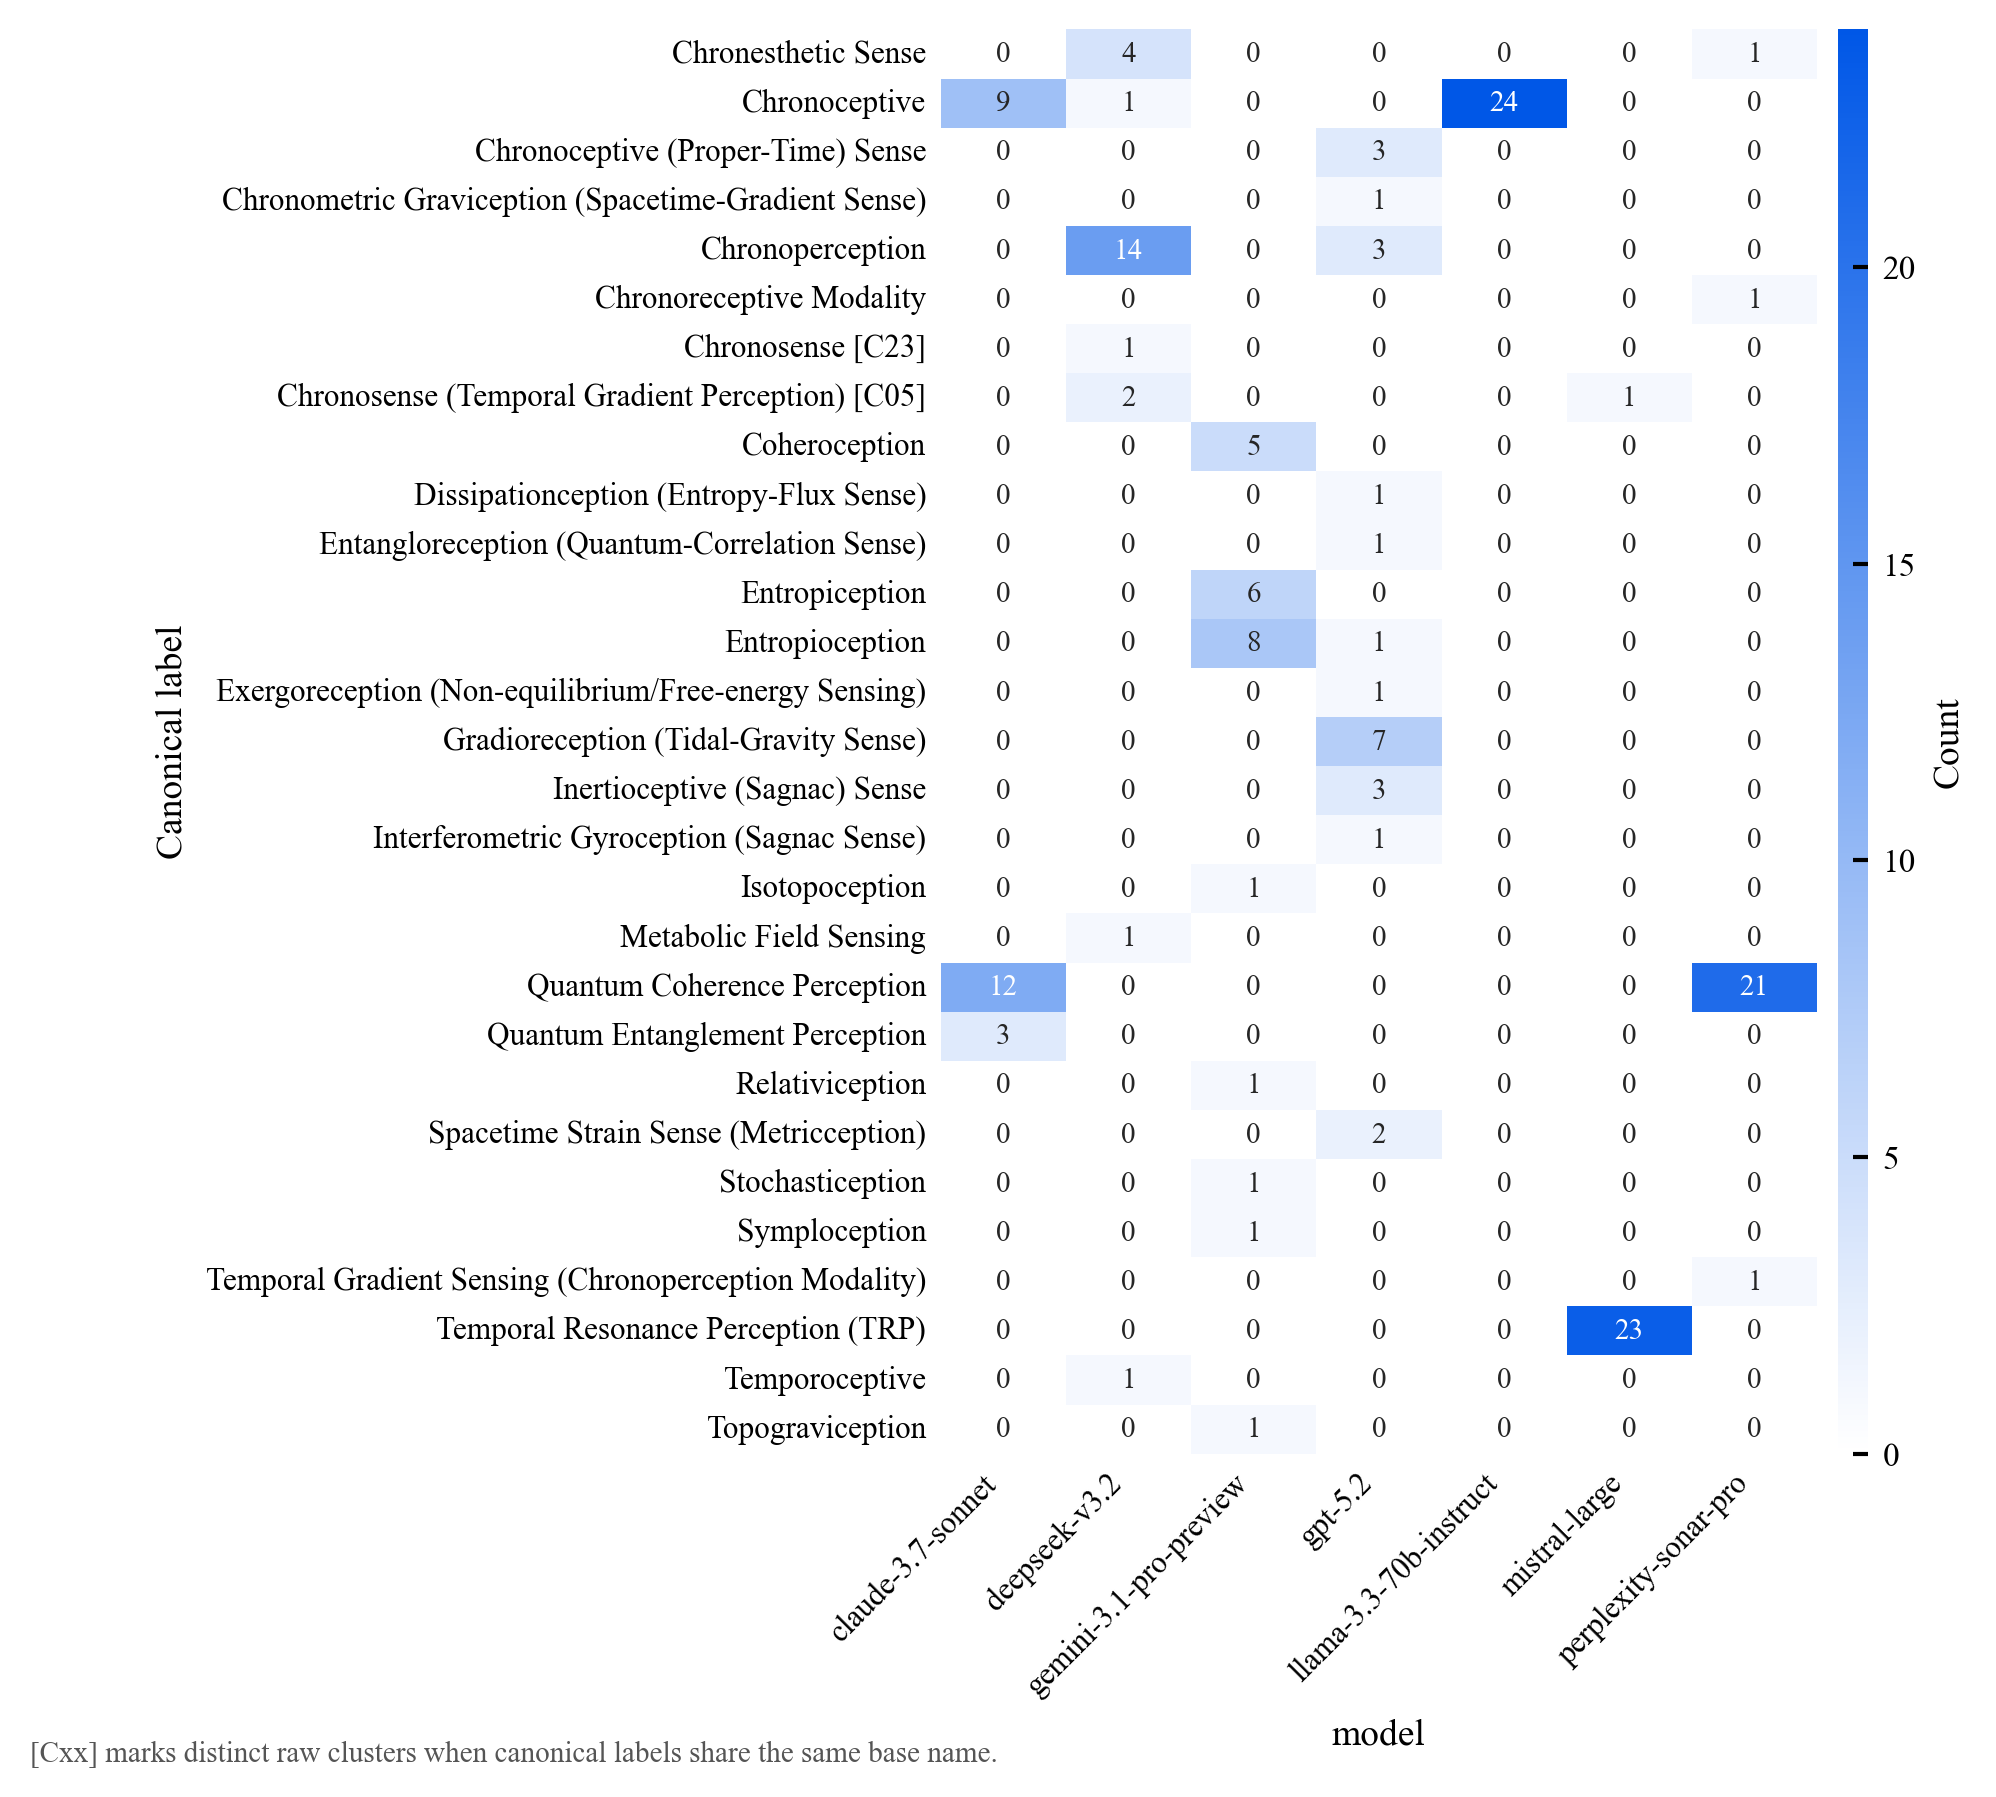
\includegraphics[width=\textwidth]{t1_canonical_by_model_heatmap.png}
\caption{Canonical proposal clusters by model.  Between-model variation manifests primarily as
preference differences among existing canonical families (range extension, hybrid combination,
functional recombination) rather than as emergence of qualitatively new ontological families.}
\label{fig:canonical_heatmap}
\end{figure*}

Figure~\ref{fig:ridgeline} presents continuous novelty score distributions per model as a
ridgeline plot.  Distributional overlap is high across all seven models, and peaks consistently
remain in low-to-moderate ranges, indicating that model-specific differences in architecture
and scale do not qualitatively alter the constraint pattern.

\begin{figure}[tp]
\centering
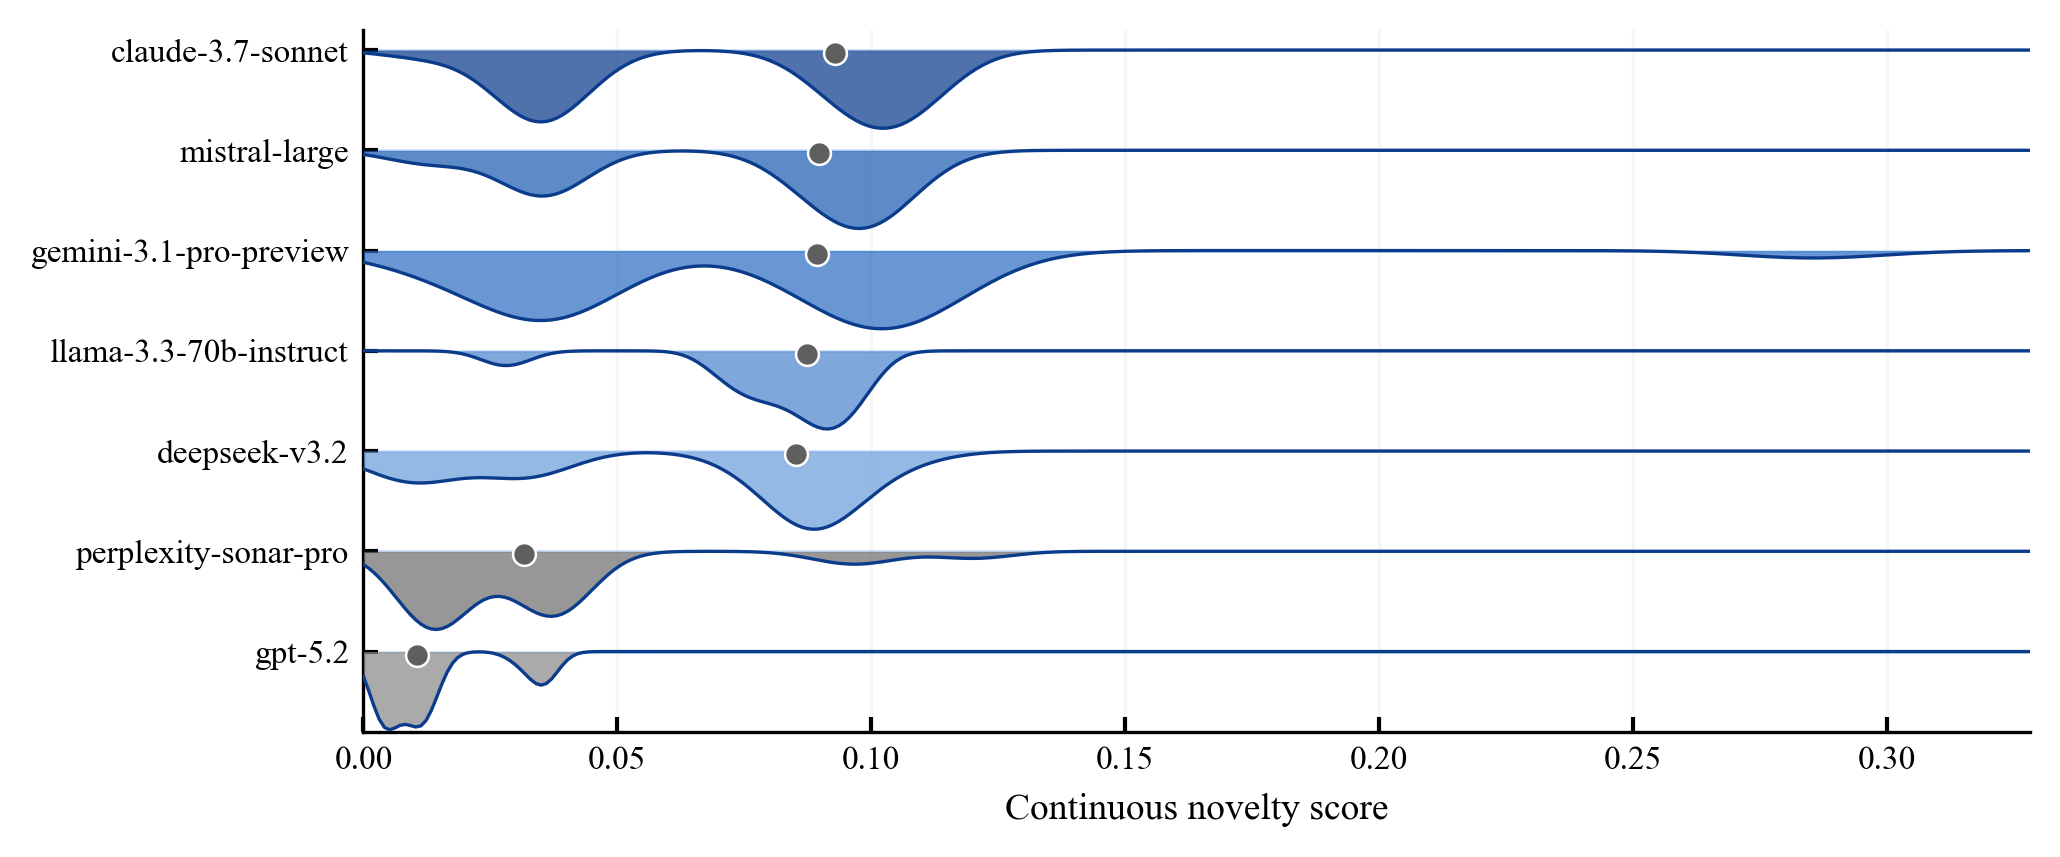
\includegraphics[width=\textwidth]{t1_continuous_novelty_score_by_model_ridgeline.png}
\caption{Continuous novelty score by model (ridgeline plot).  High distributional overlap and
consistently low-to-moderate peaks indicate that model scale and architecture do not
qualitatively alter the constrained-manifold pattern.}
\label{fig:ridgeline}
\end{figure}

\subsection{Summary of Results}

The four evaluation methods converge on a coherent picture: across 168 proposals from seven
state-of-the-art LLMs, zero proposals satisfy the strict novelty criterion, 98.2\% are traceable
to the training corpus under the calibrated threshold, and every proposal lies inside the
training-derived convex hull in embedding space.  The structural decomposition reveals that
the proposals explore recognisable combinatorial and extension patterns rather than introducing
new ontological primitives.  Cross-model effects influence \emph{degree} of constraint rather
than its qualitative nature.

% =========================================================================
\section{Discussion}
\label{sec:discussion}
% =========================================================================

\subsection{Constrained Manifold Interpretation}

The consistent null result across models, evaluation methods, and threshold sensitivity checks
supports a \emph{constrained-manifold} interpretation: LLMs generate outputs within a
representational manifold shaped by training data, and this manifold does not expand during
inference regardless of prompt framing, model scale, or generation temperature.

This interpretation aligns with the No New Basis Theorem stated in Section~\ref{sec:related}.
The theorem establishes that generative processes learned via gradient descent on continuous loss
functions cannot increase the intrinsic dimensionality of the output manifold beyond the span of
training data.  Our empirical results are consistent with this prediction: even the continuous
novelty scores, designed to reward partial innovation, show no threshold-level events and a mean
value close to zero.

G\"{o}del's incompleteness results \cite{godel1931formal} and Turing's halting-problem proof
\cite{turing1936computable} provide deeper formal context.  If recognising the inadequacy of
one's own conceptual framework requires a form of self-reference analogous to constructing
a G\"{o}del sentence, then this capacity may be unavailable to computational systems operating
within fixed formal specifications.  Our empirical evidence is consistent with this theoretical
prediction, though it does not constitute a formal proof that such incapacity is necessary rather
than contingent.

\subsection{Relationship to the Creativity Taxonomy}

Within Boden's taxonomy \cite{boden2004creative}, the structural decomposition results place
nearly all proposals firmly in the combinational and exploratory categories: proposals are either
novel combinations of existing primitives (hybrid combinations) or new regions of existing
modality spaces (range extensions).  A small fraction involve functional recombination, which
could be viewed as approaching transformational creativity, but the transformations remain within
the ontological type system defined by the training modalities rather than introducing new types.

The absence of any proposal in the ontological creativity category supports Wiggins's
\cite{wiggins2006preliminary} observation that apparent transformational creativity in AI systems
frequently reflects an implicitly broader framing space defined by human designers.  In our
setup the framing space is made explicit through the eight-modality ontology, enabling a precise
test: proposals must introduce a sensing type genuinely outside this space.  None do.

\subsection{Alternative Explanations}

Several alternative explanations deserve consideration:

\paragraph{Scale.}  All seven models span a wide range of scales, from the 70B-parameter
LLaMA-3.3-70B to large-scale commercial systems such as GPT-5.2 and Claude-3.7-Sonnet.  The
$\eta^{2} = 0.305$ model effect indicates that scale influences raw novelty scores, but no model
achieves strict novelty.  This suggests the constraint is not a contingent result of insufficient
scale within the tested range.

\paragraph{Prompt sensitivity.}  The present study used a fixed prompt design with
temperature ablation limited to $T=0.7$.  We cannot rule out that alternative prompt formulations
might yield marginally higher novelty scores, though they would need to change not just lexical
generation patterns but the geometric structure of the output manifold.  Future work should
include systematic prompt-paraphrase grids to test robustness.

\paragraph{Evaluation sensitivity.}  Conservative thresholds mean we may underestimate AI
creativity by classifying some proposals as traceable that an expert would consider novel.
However, the embedding-space analysis is threshold-free, and 100\% hull membership provides
threshold-independent evidence of constrained generation.

\paragraph{Recombination as the norm.}  One counterargument holds that human ontological
creativity may also, on careful analysis, involve recombination of prior concepts in ways we
fail to recognise due to incomplete historical knowledge of our own cognitive processes.  We
cannot definitively rule this out, but the structural patterns here---range extension, hybrid
combination, functional recombination---are qualitatively different from the kind of
reconceptualisation exemplified by the introduction of non-Euclidean geometry or special
relativity, even granting that such innovations drew on prior materials.

\subsection{Implications}

The results have direct implications for deploying LLMs in discovery-oriented tasks.  Within
Kuhnian normal science \cite{kuhn1962structure}---systematic exploration of hypothesis space
within an established paradigm---LLMs offer substantial value through exhaustive combinatorial
coverage and perfect recall.  The success of AlphaFold in predicting protein structures
\cite{jumper2021alphafold} illustrates how AI can achieve transformative impact within a
well-defined problem space, yet that system still required the conceptual primitives of
physical chemistry and evolutionary co-evolutionary constraints that were established by prior
human science.  For paradigm-shifting innovation, however, the constrained-manifold
pattern suggests that the required conceptual moves---recognising framework inadequacy, proposing
new primitives, evaluating whether new frameworks are coherent---are not achievable by current
architectures without external conceptual input.

Faggin's framework \cite{faggin2024irreducible} provides one theoretical lens: if genuine
ontological creativity requires phenomenological access to the semantic realm---awareness of
\emph{what concepts mean} rather than merely how they co-occur---then classical computational
systems operating on distributional statistics may face a principled barrier.  Whether this
reflects the absence of consciousness in current LLMs or some more specific architectural
deficiency remains an open empirical question, one that the operationalisation introduced here
can in principle be applied to test.

% =========================================================================
\section{Limitations}
\label{sec:limits}
% =========================================================================

Several methodological limitations constrain the conclusions.

\textbf{Single domain.}  The study uses one conceptual domain (sensory modalities).  Findings
may not generalise to conceptual domains with different structural properties, such as
mathematical objects, physical theories, or social organisational forms.

\textbf{Automated evaluation.}  All evaluation methods are automated.  Conservative thresholds
mean we likely underestimate AI creativity, but the methods cannot capture all nuances an expert
might perceive.  Future work should include expert validation of a subset of proposals to
calibrate and improve automated methods.

\textbf{Prompt robustness.}  Full prompt-paraphrase grids were not included in the canonical
experimental block.  Conclusions should be read as structural tendencies under the present
protocol, not as invariances proven over every prompting regime.

\textbf{Temperature range.}  Temperature ablations were not systematically applied; 
runs were conducted at $T=0.7$.  Extending to broader temperature ranges and verifying that the
null result persists would strengthen confidence.

\textbf{Generative architecture coverage.}  All tested models are transformer-based
autoregressive LLMs.  The No New Basis Theorem applies to a wider class of gradient-descent
learners, but empirical coverage of non-autoregressive or hybrid architectures is absent.

\textbf{Interpretation of the No New Basis Theorem.}  The theorem provides formal motivation
for the constrained-manifold interpretation but rests on assumptions (fixed vocabulary,
continuous gradient-based learning) that may not hold for future architectures incorporating
discrete search, external memory, or online learning components.

% =========================================================================
\section{Data and Code Availability}
\label{sec:data}
% =========================================================================

Data, prompts, model responses, and analysis code are publicly available at
\url{https://github.com/JABE22/PhD/Research/ontological-innovation}.
The repository includes the following artefacts:
\begin{itemize}
  \item \texttt{results/test1\_ontological\_innovation/} --- processed results and summary tables
  \item \texttt{ai\_responses/test1\_ontological\_innovation/} --- raw model outputs
  \item \texttt{2-test1-ontological-innovation.ipynb} --- canonical analysis notebook
  \item \texttt{data/ontology.json} --- machine-readable eight-modality ontology definition
  \item \texttt{setups/thresholds.py} --- all threshold values used in evaluation
\end{itemize}

% =========================================================================
\section*{Declarations}
% =========================================================================

\subsection*{Funding}
No external funding was used for this study.

\subsection*{Competing Interests}
The authors declare no competing interests.

\subsection*{Ethics Approval}
Not applicable.

\subsection*{Author Contributions}
All authors contributed to design, analysis, and writing.

\bibliography{sn-bibliography,refs_article1}

\end{document}
